%%%%%%%%%%%%%%%%%%%%%%%%%
% Closure tests
%%%%%%%%%%%%%%%%%%%%%%%%%

In this analysis, we do not explicitly estimate the background in the signal region from the
observations in the control regions. Rather, we create a prior distribution for the four background
components of the signal regions, that incorporates all statistical and systematic uncertainties, as
will be described in detail in Section~\ref{sec:boost_likelihood}. 
However, in order to verify that the control regions defined in the previous sections provide
adequate data-driven models for the backgrounds in the signal region and that the translations
between different regions behave as expected, we perform two cross checks, taking into account
statistical uncertainties only. 

\subsubsection{First cross check}

In the first cross check, we predict the background in a signal-like control region, denoted by
$S^\prime$, defined by inverting the $\Delta\phi_{min}$ requirement while preserving the rest of the
selection, see Table~\ref{tab:boost_selection_summary}. 
The estimated number of events in the $S^\prime$ region for the QCD multijet, $\W(\rightarrow
\ell\nu)+$jets, and $t\bar{t}$ (plus single top) processes is computed from the observations in the 
$Q$, $T$, and $W$ regions as follows,
\begin{equation}
 \widehat{N}_{\rm QCD}^{S^\prime} = \left( N_{\rm obs}^{Q} - N_{{\rm other, MC}}^{Q} \right)  /
\left(
\frac{N_{\rm QCD}^{Q}}{N_{\rm QCD}^{S^\prime}} \right)_{\rm MC},
\label{eq:E1}
\end{equation}
\begin{equation}
 \widehat{N}_{\W\ell\nu}^{S^\prime} = \left( N_{\rm obs}^{W} - N_{\rm other, MC}^{W} \right) /
\left(
\frac{N_{\W\ell\nu}^{W}}{N_{\W\ell\nu}^{S^\prime}} \right)_{\rm MC},
\label{eq:E2}
\end{equation}
\begin{equation}
  \widehat{N}_{\rm TTJ+T}^{S^\prime} = \left( N_{\rm obs}^{T} - \widehat{N}_{\rm QCD}^{T} - N_{\rm
other, MC}^{T}
\right) / \left( \frac{N_{\rm TTJ+T}^{T}} {N_{\rm TTJ+T}^{S^\prime}}\right)_{\rm MC},
\label{eq:E3}
\end{equation}
while the estimated number of multijet events in the top control region is given by,
\begin{equation}
 \widehat{N}_{\rm QCD}^{T} = \left( N_{\rm obs}^{Q} - N_{\rm other, MC}^{Q} \right) /  \left(
\frac{N_{\rm QCD}^{Q}}{N_{\rm QCD}^{T}} \right)_{\rm MC}.
\label{eq:E4}
\end{equation}
As can be seen from Table~\ref{tab:cutflow}, $N_{QCD, {\rm MC}}^{T} = 0$ for the nominal choice of
systematic uncertainties. The formulae above can thus be simplified since $\widehat{N}_{QCD}^{T} =
0$. This is, however, not necessarily the case for other choices of systematic variations. This
relation is, therefore, still used to constrain the expected multijet background in the $T$ region
during the final background estimate. 
The total estimated background in the $S^\prime$ region is
\begin{equation}
  \hat{N}^{S^\prime} = \sum_i \hat{N}^{S^\prime}_i , 
\end{equation}
where $i$ runs over all background processes.  For the smaller backgrounds, $\hat{N}^{S^\prime}_i$
is determined by simulation. 
The estimation of backgrounds is done bin-by-bin in the $(\mr,\rsq)$ space. 
However, the estimated scale factors are global as the statistical precision is not sufficient to
yield reliable bin-by-bin estimates. The expected global scale factors, which we denote by $\kappa$,
 are defined in Section~\ref{sec:boost_likelihood}, which also describes how they are calculated.

Figure~\ref{fig:Shape_syst_1D_project_sideband} shows the projection on the $\mr$ and $\rsq$ axes of
the predicted and observed distributions.  The prediction agrees with observation within 20\%.  This
cross check of the background modelling shows that it is feasible to estimate a multicomponent 
background in a signal-like region using the control regions we have defined.
In this test, aspects of the MC modelling, such as $\cPqb$ tagging, translation between lepton 
multiplicities, and certain aspects of the $\W$ tagging, have been verified. 

\begin{figure}[htpb]
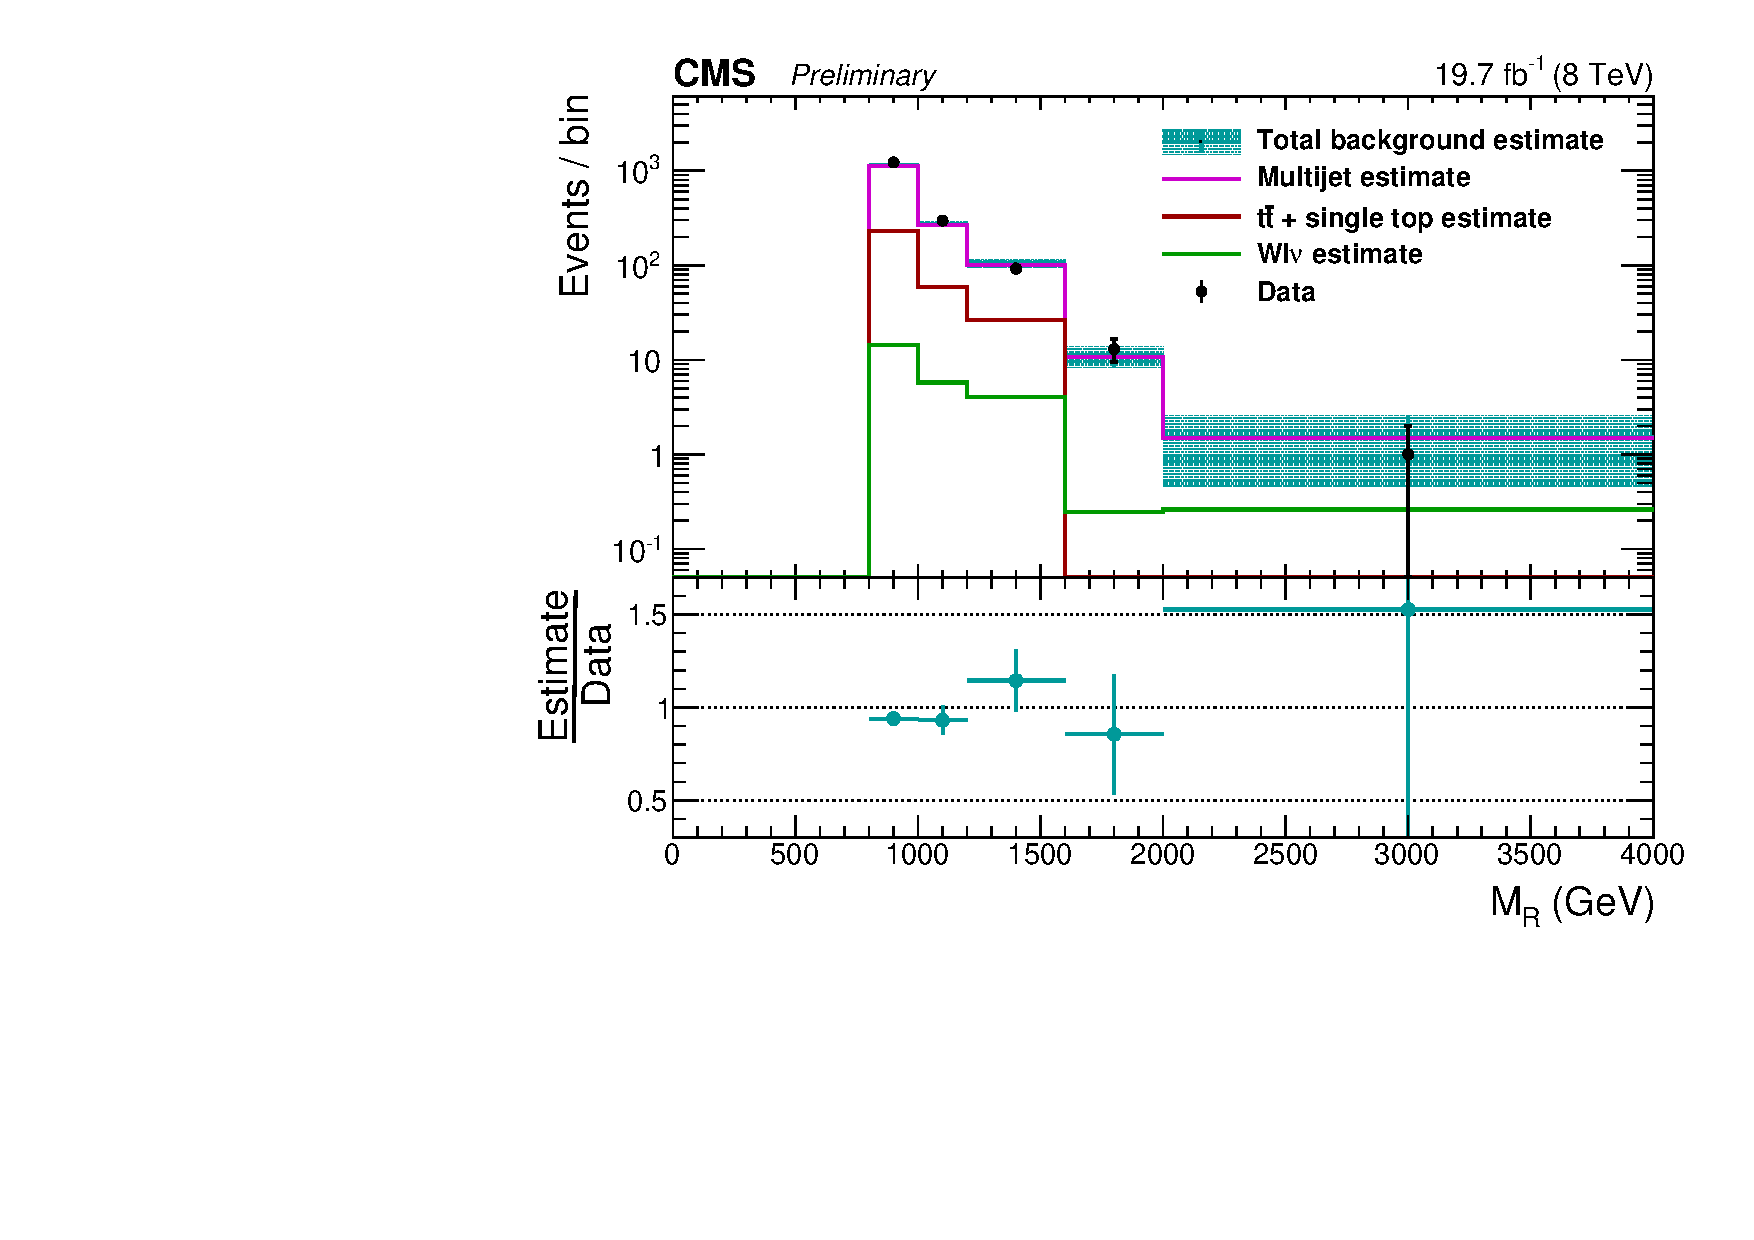
\includegraphics[width=0.48\textwidth]
{figures/razor_selection/MR_comparison_data_estimate_g1Mbg1W0Ll_mdPhi0p5_log}
~
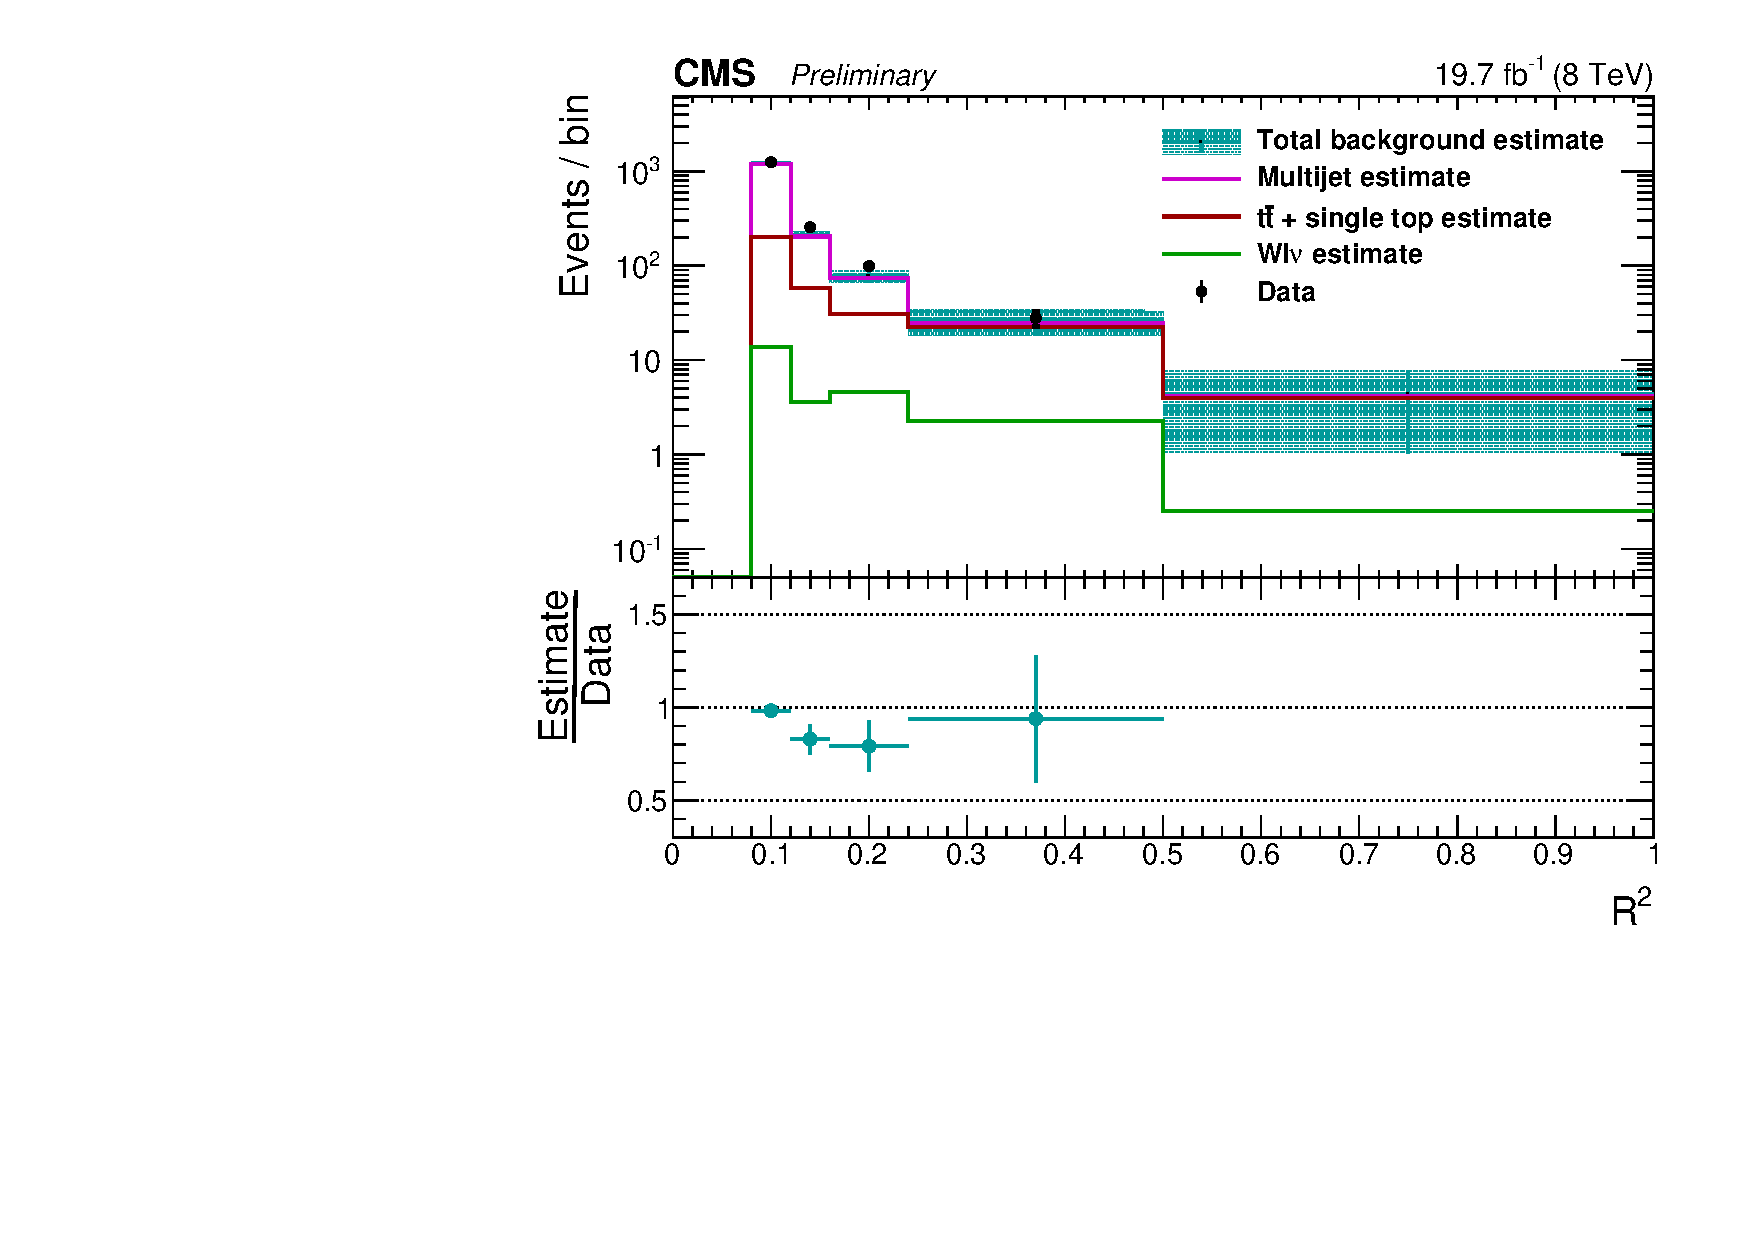
\includegraphics[width=0.48\textwidth]
{figures/razor_selection/R2_comparison_data_estimate_g1Mbg1W0Ll_mdPhi0p5_log}
\caption{1D projection of $\mr$ (left) and $\rsq$ (right) for the closure test predicting the
$\Delta\phi_{min}$ sideband region $S'$. The uncertainties shown are statistical only and the
horizontal error bars only indicate the bin width.
\label{fig:Shape_syst_1D_project_sideband}}
\end{figure}


\subsubsection{Second cross check}

In a second cross check, we use the $Q$ region to estimate the background in a more signal-like $Q$
region, denoted by $Q^\prime$, where $\Delta\phi_{min} > 0.5$, from the relationship
\begin{equation}
  \hat{N}^{Q^\prime} = N_{\rm obs}^Q \frac{N_{\rm MC}^{Q^\prime}}{N_{\rm MC}^Q}.
\end{equation}
Here $N_{\rm MC}$ includes all contributing simulated background processes, and $N_{\rm obs}^Q$ is
the observed data count in the $Q$ region.
This test assesses the degree to which the simulated distribution of $\Delta\phi_{min}$ as well as
its extrapolation from the $Q$ region to the $S$ region are reliable. The comparison between
prediction and observation is shown in Fig.~\ref{fig:Shape_syst_1D_project_QCD}.
The level of discrepancy (${\sim}\,40\%$) between the prediction and observation in this cross check 
is incorporated as a systematic uncertainty in the global scale factors, as described in
Section~\ref{sec:boost_likelihood}.

\begin{figure}[htpb]
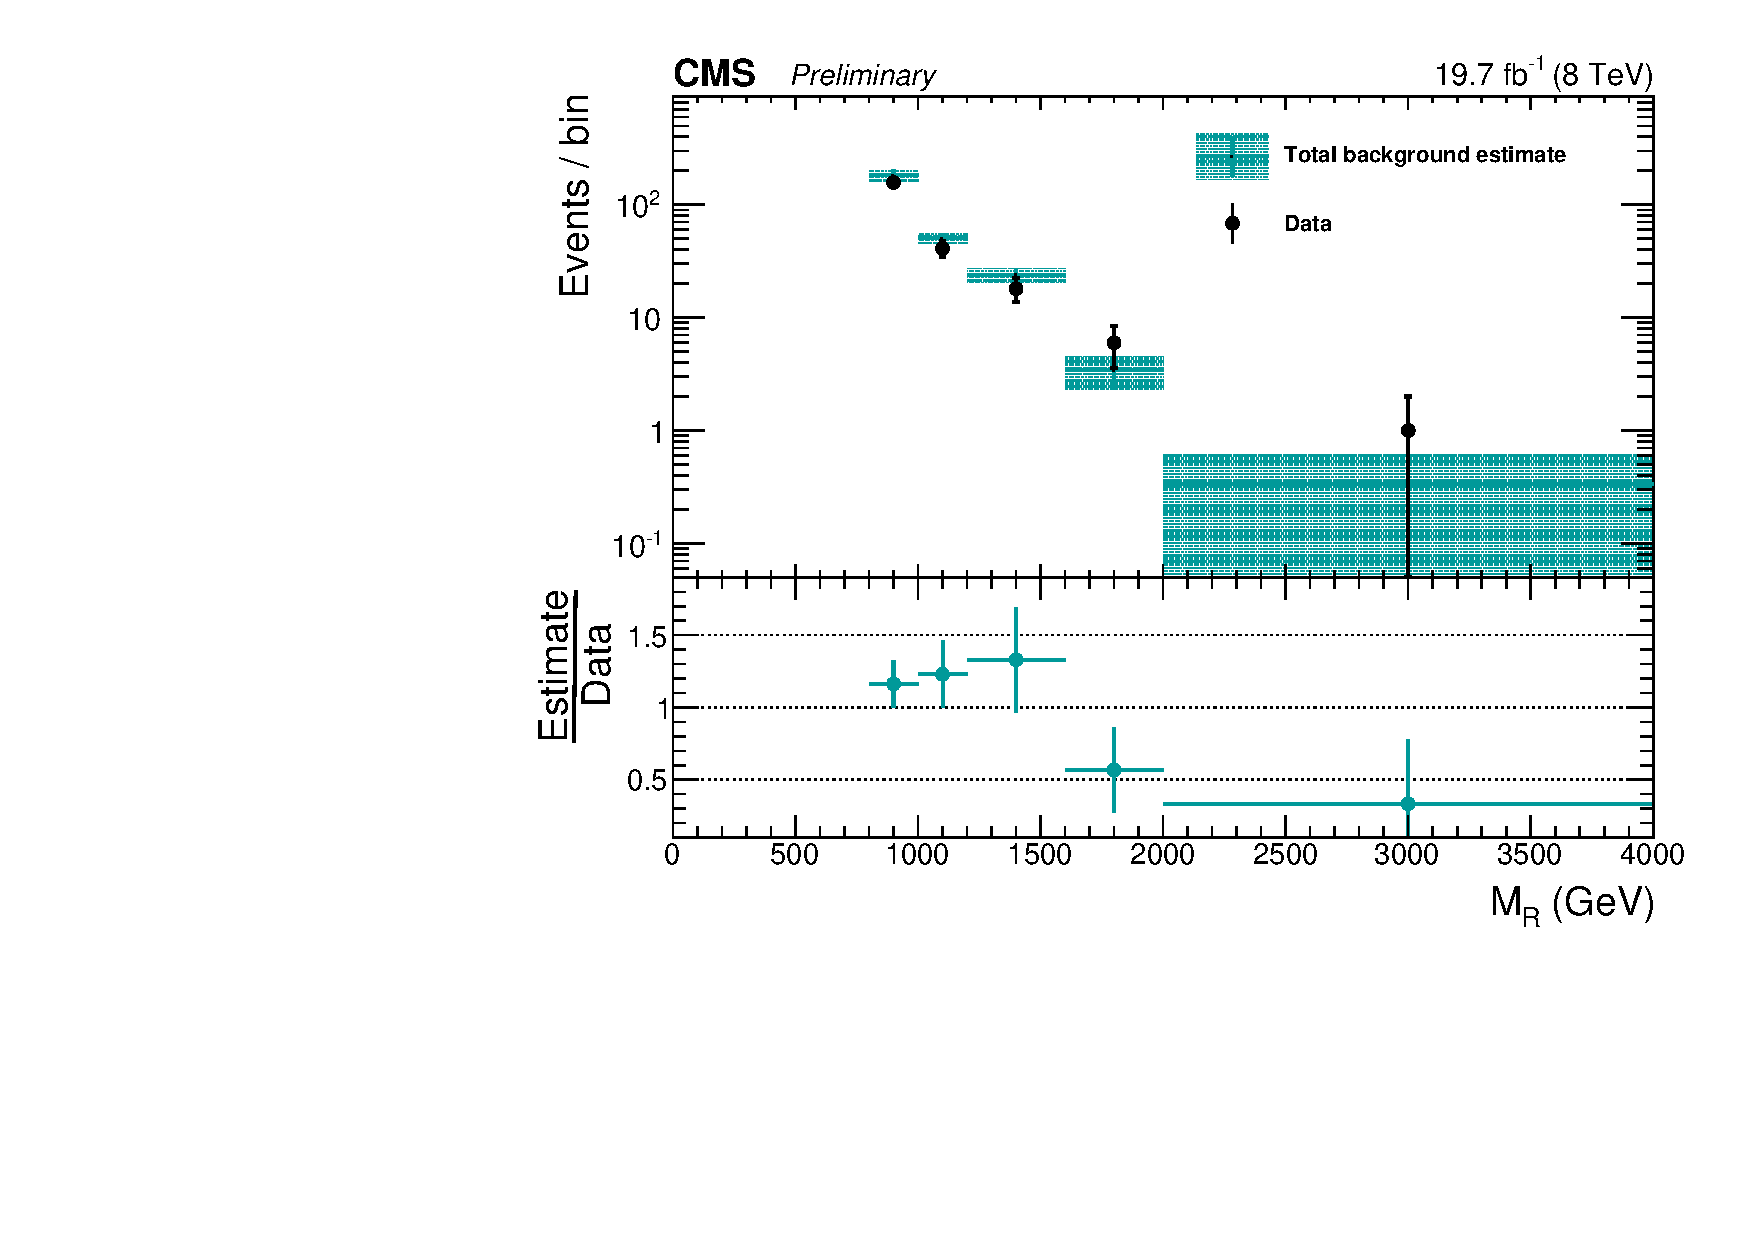
\includegraphics[width=0.5\textwidth]
{figures/razor_selection/MR_comparison_data_estimate_0Lbg1uW0Ll_mdPhig0p5_from_0Lbg1uW0Ll_mdPhi0p3_log}
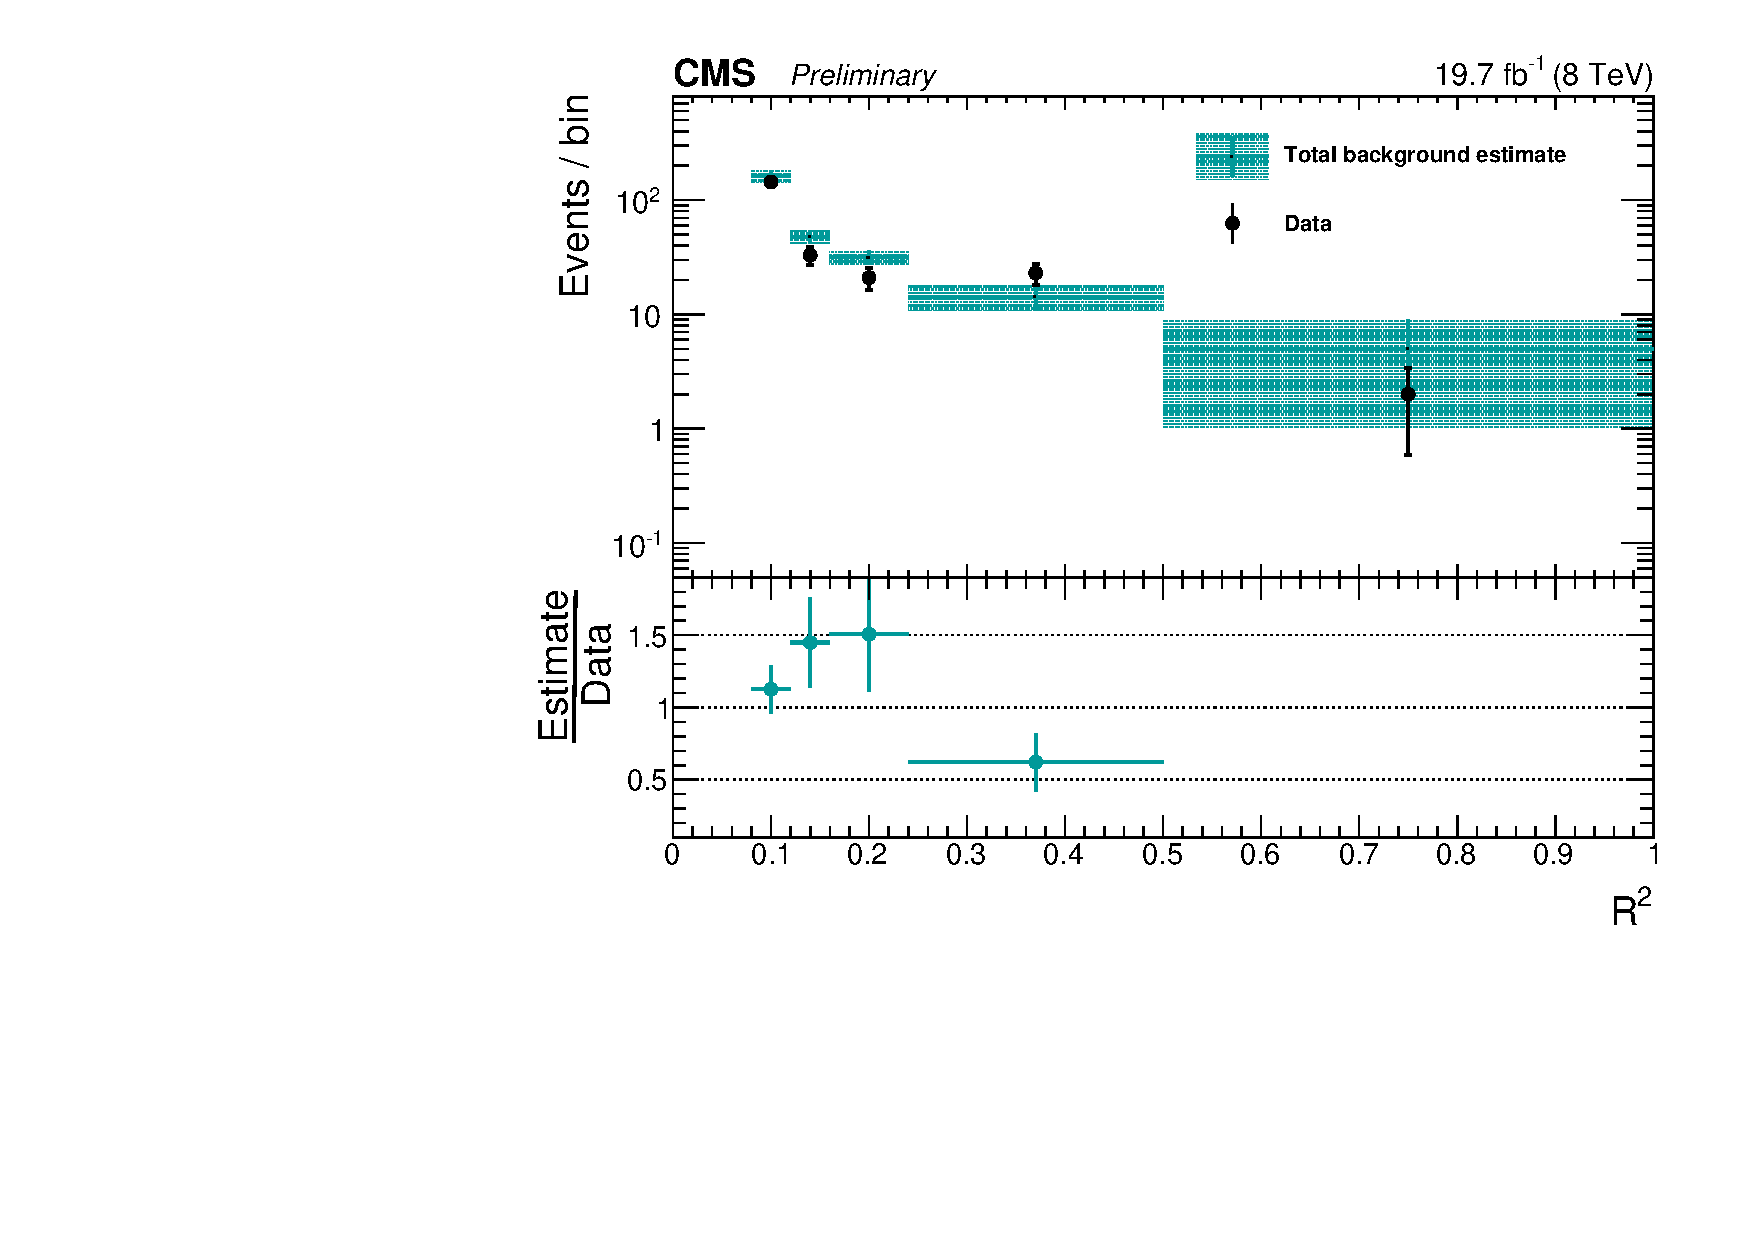
\includegraphics[width=0.5\textwidth]
{figures/razor_selection/R2_comparison_data_estimate_0Lbg1uW0Ll_mdPhig0p5_from_0Lbg1uW0Ll_mdPhi0p3_log}
\caption{1D projection of $\mr$ (left) and $\rsq$ (right) for the closure test predicting the
background in region $Q'$, as defined in the text. The uncertainties shown are statistical only
and the horizontal error bars only indicate the bin width.
\label{fig:Shape_syst_1D_project_QCD}}
\end{figure}
